\begin{figure}[t]
    \centering
    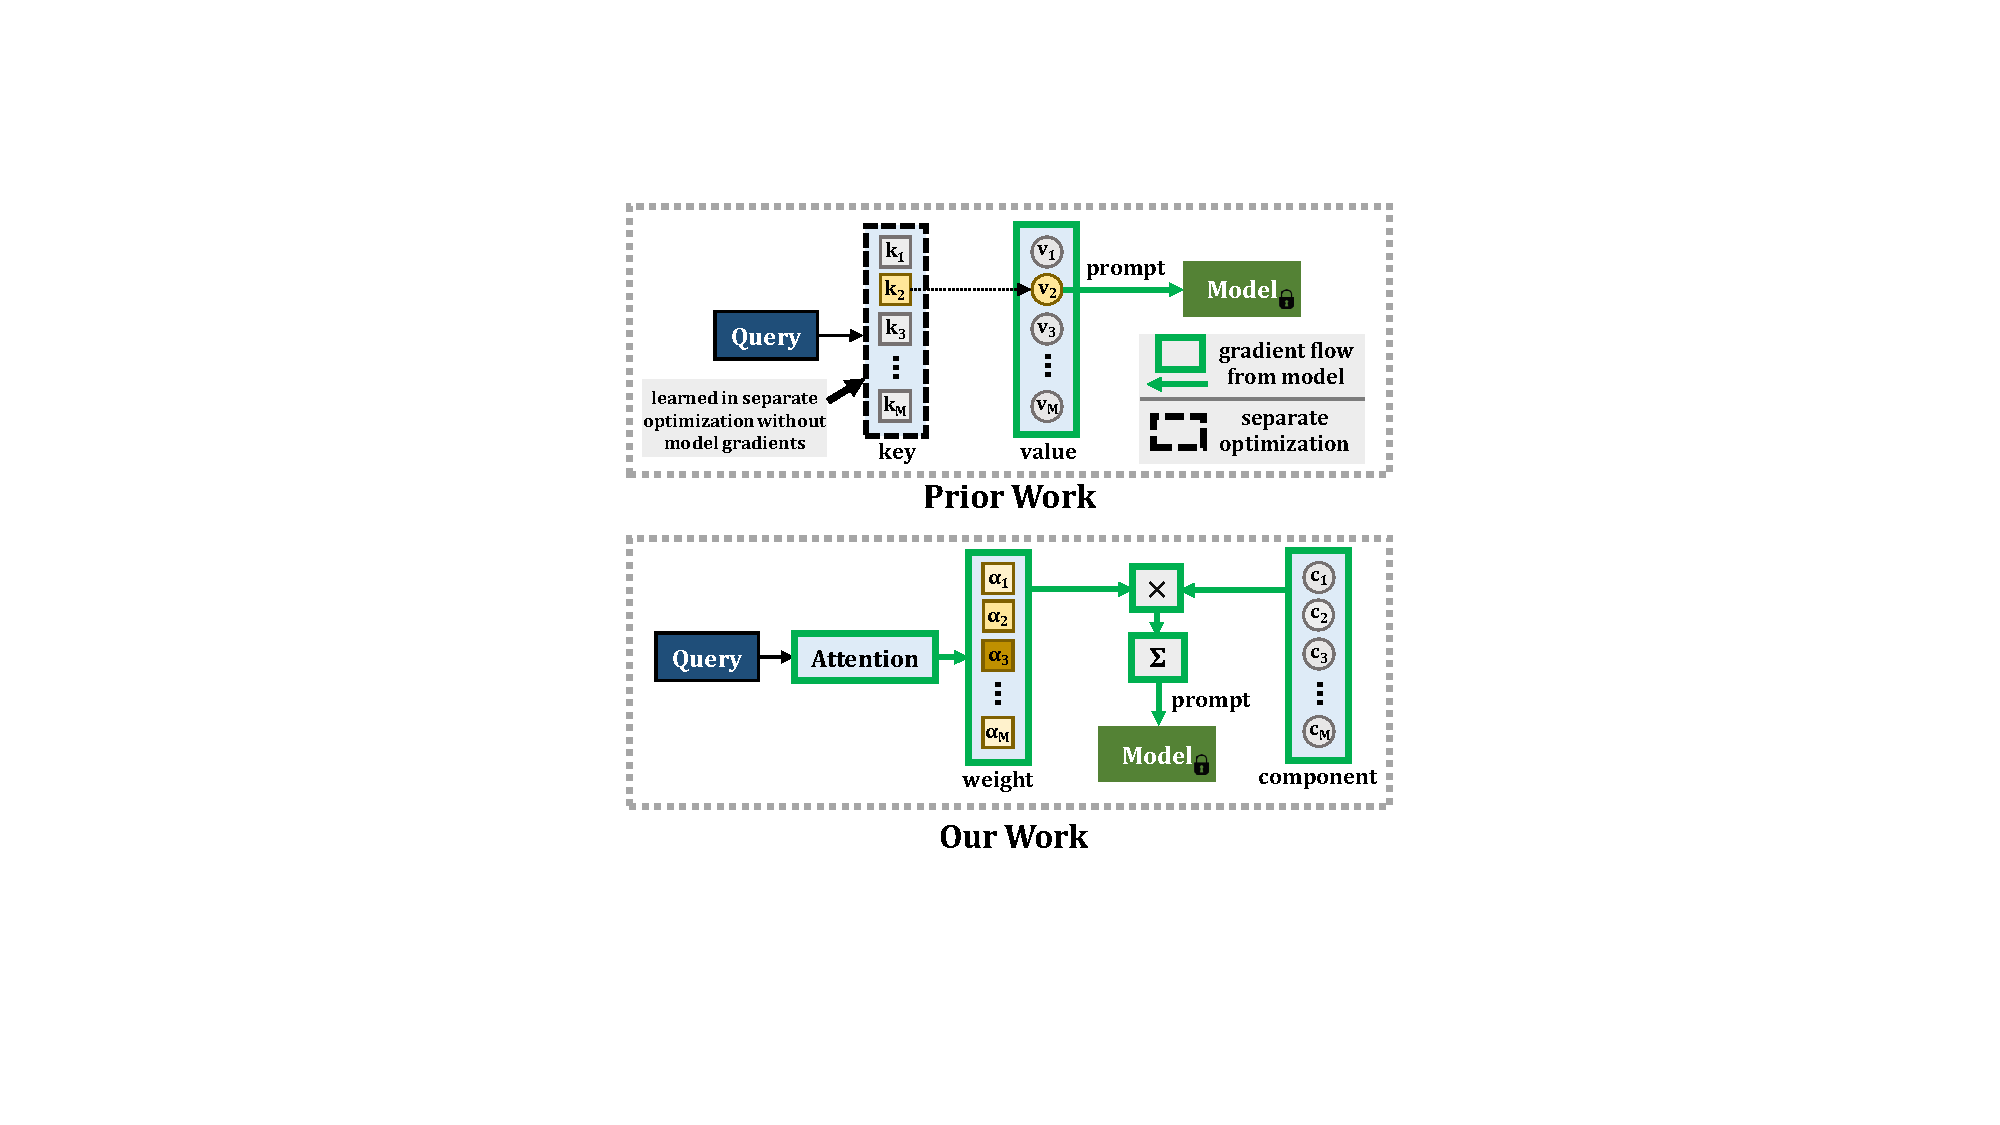
\includegraphics[width=0.46\textwidth]{figures/source/key_idea.pdf}
    \caption{\textbf{Prior work}~\cite{wang2022dualprompt} learns a pool of key-value pairs to select learnable prompts which are inserted into several layers of a pre-trained ViT (the prompting parameters are unique to each layer). \textbf{Our work} introduces a \textbf{decomposed prompt} which consists of learnable prompt \emph{components} that assemble to produce \emph{attention-conditioned} prompts. Unlike prior work, ours is \textbf{optimized in an end-to-end fashion} (denoted with thick, green lines).
    }
    \label{fig:key-idea}
    \vspace{-3mm}
\end{figure}




